\section{Some examples}
\label{sec:gamesforld}
	% (Apresentar exemplos de trabalho relacionado)
	% (Procurar por jogos idênticos que tratem o mesmo problema)

Before the development of the games themselves, we should first look into some other existing solutions. This will allow for some advantages as we can analyse each one, knowing which characteristics are better suited for the mini-games being developed in this thesis.
As we are developing different games targeted for different age groups and disabilities, we will have to group our research for games that aim to help for each \gls{ld}. This way, we can capture some characteristics for each game and it will be easier when developing each mini-game from scratch.
Next, we'll present some of the games found that can be useful for the research.

\newpage
\subsection*{Fast ForWord} 

Fast ForWord\cite{fastforword} is a game that helps children will \textbf{dyslexia} and \textbf{Language Processing Disorder} to improve their phonological awareness, auditory processing and skills. It uses adaptive technology to provide individualized feedback and instruction.
Fast  ForWord is based on the neuroscience principles of neuroplasticity, the ability of the brain to change and adapt in response to stimulation and learning. It consists of two phases: cognitive and reading. The cognitive phase works on skill gaps and building fundamentals, such as processing, working memory, attention, and sequencing. The reading phase trains reading fluency and comprehension as well as vocabulary, grammar, and syntax. It has 9 programs in total each with 5-7 exercises that target different aspects of learning and reading. Each program is designed for different age groups and levels of difficulty.
According to a meta-analysis of over 300 efficacy and research studies, Fast ForWord users achieved an average gain of 2 years in reading skills in about 6 months. \cite{gemlearningFastFor}
One of the games consists of listening to a story and then answering questions and following instructions. This improves skills in listening comprehension and builds familiarity with English language conventions. Figure \ref{fig:fastforword} shows the aspect of this game in specific.

\begin{figure}[!h]
    \centering
    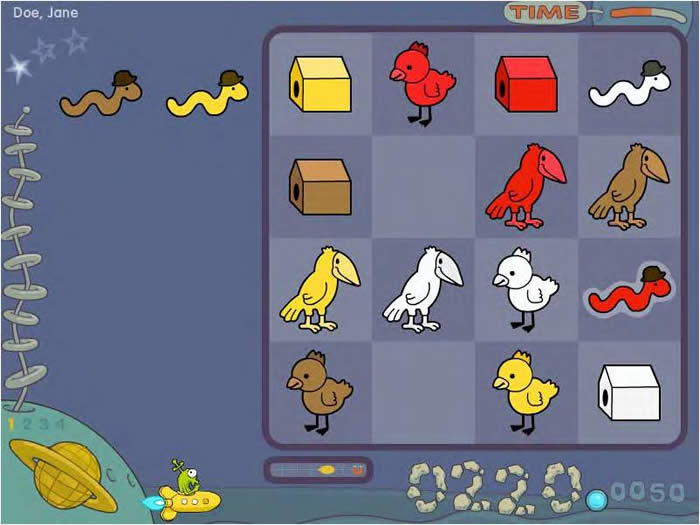
\includegraphics[width=0.8\linewidth]{Chapters/related_work_img/FastForWord_Cosmic_Reader.jpg}
    \caption{Fast ForWord - Cosmic Reader}
    \label{fig:fastforword}
\end{figure}
% https://www.gemmlearning.com/programs/fast-forword/

% https://www.apa.org/topics/learning-memory/dyslexia-video-games
% https://www.scilearn.com/ - Game Site

% https://www.apa.org/topics/learning-memory/dyslexia-video-games
% https://www.unicef.org/parenting/child-care/10-playful-educational-activities-children-disabilities
% https://www.parentcircle.com/games-and-activities-for-special-needs-and-autistic-children/article
% https://www.commonsensemedia.org/articles/5-ways-video-games-can-help-kids-with-disabilities
% https://parentingpod.com/dyslexia-activities/


\subsection*{NumberShire} 

NumberShire \cite{numbershire} is an internet-based game that aims at educationg children with intense focus on critical whole number concepts and skills for students. It is made for all students, but specially for those with difficulties in mathematics. This directly impacts children with dyscalculia and other math-related \glspl{ld}.

It was developed with support from the U.S Department of Education. It achieved great results in several controlled trials, with students having significant gains in their math skills, against students with typical math support.

The game is composed of mathematical concepts in a story-based, fantasy setting. Players complete quests by solving math problems tailored to their specific skill level. Through this narrative, children learn foundational math concepts such as addition, subtraction, and number sense. The game provides immediate feedback and rewards progress, creating a motivational framework that encourages practice.

Figure \ref{fig:numberShire} details the visual representation of the gameplay.

\begin{figure}[!h]
    \centering
    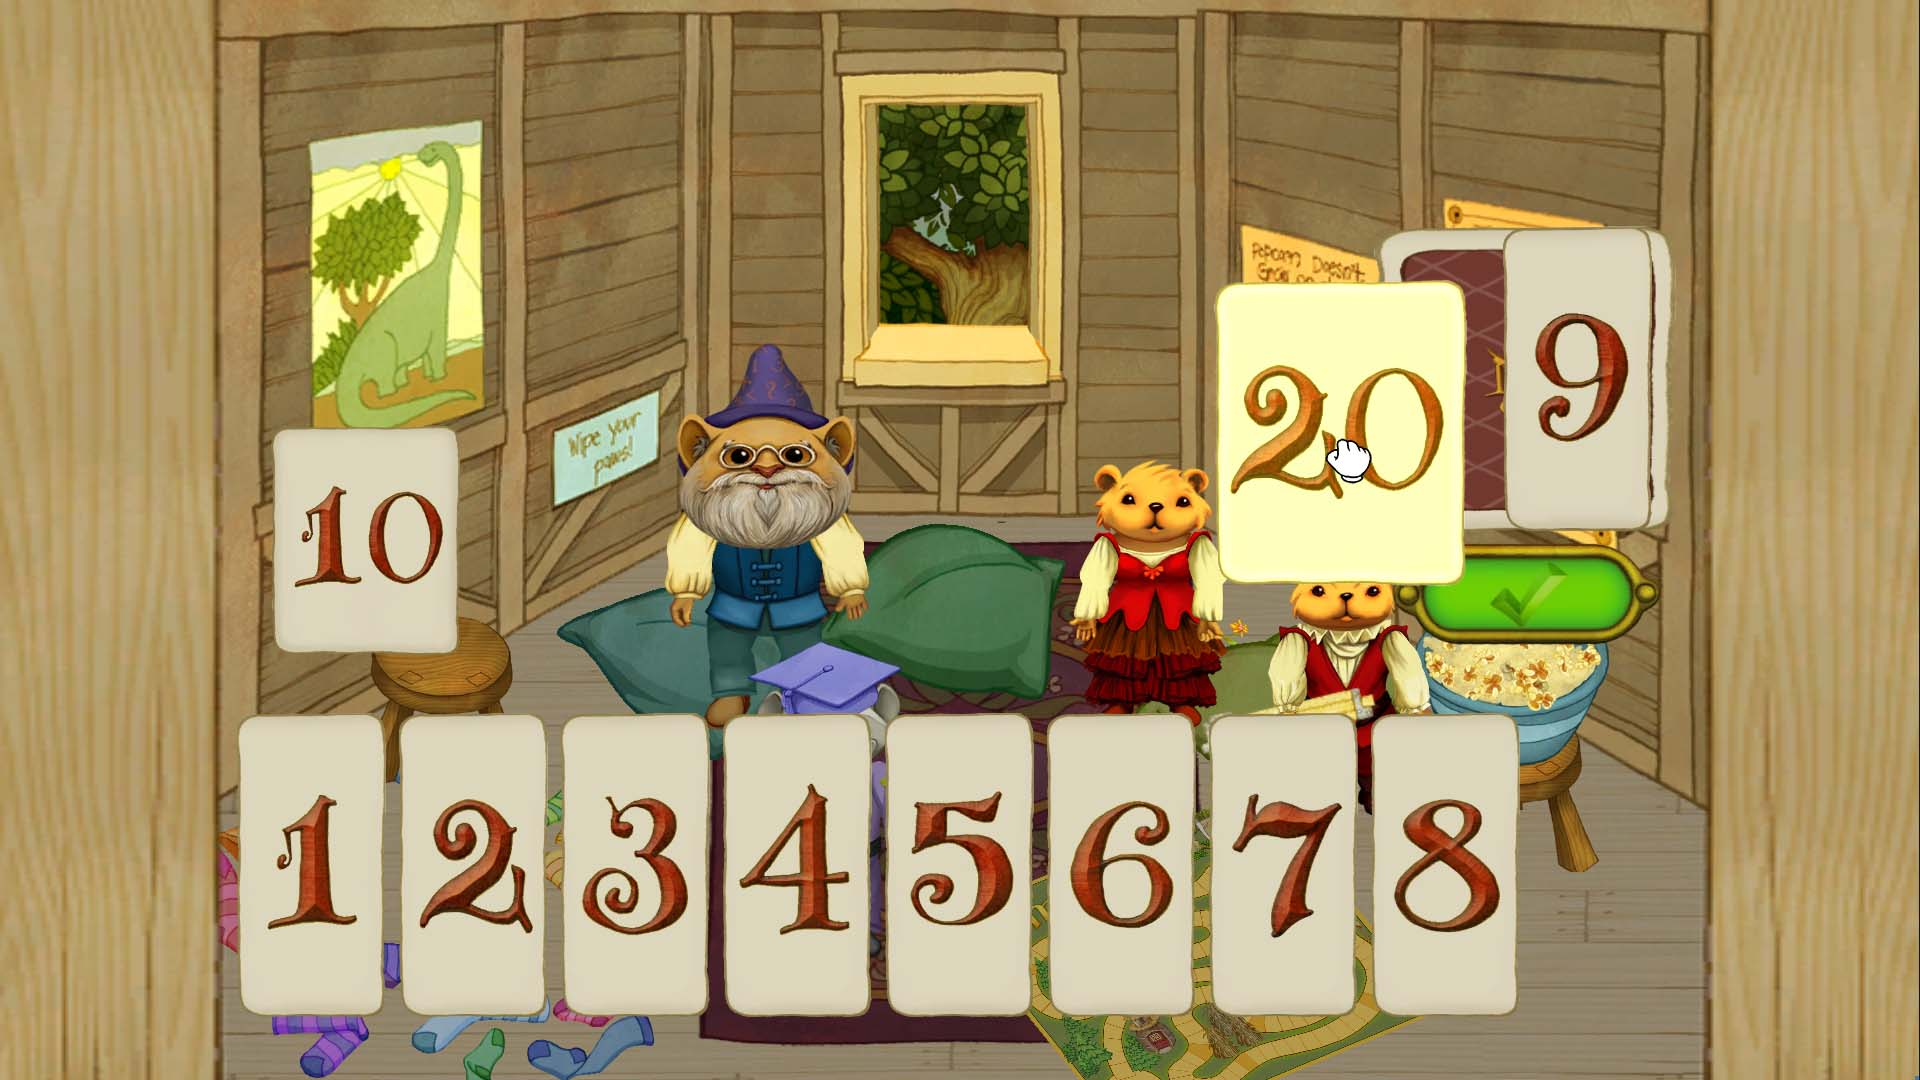
\includegraphics[width=0.8\linewidth]{Chapters/related_work_img/NumberShire_gameplay02.jpg}
    \caption{NumberShire - Gameplay}
    \label{fig:numberShire}
\end{figure}


\subsection*{GraphoGame}
% The best results have been found in children aged 5 to 8, although - in practice - it is useful for struggling readers of any age and children as young as 4. 

GraphoGame \cite{graphogamesoftware} is an educational game developed by a Finnish company. The game is meant to be played on touch-screen devices such as smartphones or tablets.

In the game, players create their own avatar and start to train from the most fundamental skills. It starts with letter recognizing, connecting letters with sounds. After that, children start to do letter combinations, combining sounds into syllabes and, lastly they move to challenging syllabes and complicated words. This sequence is know as the synthetic approach to reading instruction.

The game adapts in real-time to the child’s performance, offering more challenging or simplified content based on their success rate. This adaptive nature is particularly beneficial for children with dyslexia, as it allows for targeted practice on challenging areas without overwhelming the learner.

Studies on GraphoGame have found best results in children aged from five to eight years old. However it can be useful for readers of any age.

Figure \ref{fig:graphogame} displays one of the challenges inside the game.

\begin{figure}[H]
    \centering
    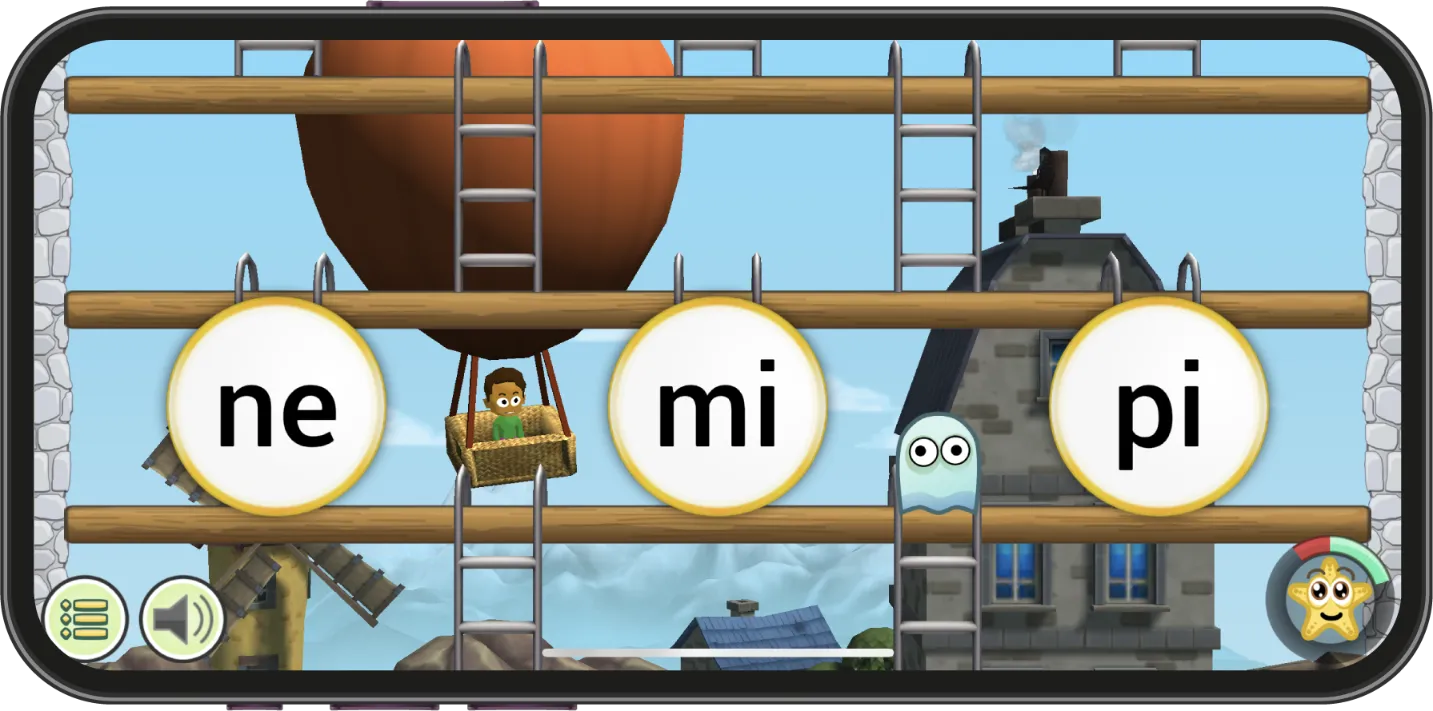
\includegraphics[width=0.8\linewidth]{Chapters/related_work_img/graphogamegameplay.png}
    \caption{GraphoGame - Gameplay}
    \label{fig:graphogame}
\end{figure}